\chapter{Raw and XML digital signature and encryption}
\section{PKCS\#7 and CMS}
PKCS\#7 is the original standard from RSA, since RSA was the owner of
the RSA algorithm, they wanted also to define standards about the
usage of the algorithm, and they had a series of standards named PKCS.

PKCS\#7 was a standard for secure enveloping (secure is a generic
term, it means authentication, integrity, confidentiality and so on),
at some point in v1.5, the work was shared with IETF and later RSA
stopped the development of PKCS\#7 and the rest was developed directly
by IETF which renamed it in CMS (Cryptographic Message Syntax).

\begin{boxH}
  CMS is a \textbf{secure envelop} that allows data authentication,
  integrity and, optionally, privacy, with symmetric or asymmetric
  algorithms, depending on the kind of application.
\end{boxH}

It also supports multiple signatures (hierarchical or parallel) on the
same object, and it can include the certificates (and can include also
revocation info) to verify the signature.

PKCS\#7 and CMS are raw format, in the sense that they consider
generic data that are just binary blob/stream (sequence of bit), and
this sequence of bits is encapsulated in a secure container. It is
very important because it is the only standard that permits to sign
and encrypt any kind of data, and it is a recursive format, which is
important because there is not one format which is providing signature
and encryption, but it is possible to achieve that by making first
encryption, then that object becomes a generic data which is inserted
in another container which is providing the signature.

PKCS\#7 and CMS are defined using ASN.1 (Abstract Syntax Notation 1)
with different encoding rules (Basic Encoding Rule, BER, for most of
the standard and the Distinguished Encoding Rule, DER, only for the
signed attributes and authenticated attributes).

Initially, it was defined by RSA and then it evolved over the time:
\begin{itemize}
  \item RFC-2630 (Jun ‘99): fully compatible PKCS\#7 1.5 but with
    key-agreement (DH algorithm) and pre- shared keys
  \item RFC-3369 (Aug ‘02): adds password-based keys and an extension
    schema for generic key management and it splits the document into
    two RFCs (one for the basic structure of secure envelop and the
    other for the algorithms, so that they can evolve independently
    for the secure container)
  \item RFC-3852 (Jul ‘04): it is just a generalization, an extension
    that supports generic certificates (not very frequent to use
    something different from X.509 is used)
  \item RFC-5652 (Sep ‘09): clarifications about multiple signatures
\end{itemize}

\subsection{Algorithms for CMS}
The allowed algorithms are documented in RFC-3370:
\begin{itemize}
  \item Digest MD5, SHA-1: quite old
  \item Signature RSA, DSA (insecure without elliptic curve)
  \item Key management:
    \begin{itemize}
      \item DH for key agreement
      \item RSA for transport
      \item For symmetric wrapping 3DES and RC2
      \item Derivation PBKDF2
    \end{itemize}
  \item For encryption: 3DES-CBC, RC2-CBC
  \item For MAC: HMAC-SHA1
\end{itemize}
These algorithms were very basic and quite old, but with new RFCs the
situation improved:
\begin{itemize}
  \item For encryption: CAST-128, IDEA, AES, Camellia, SEED
  \item For digital signature RSASSA-PSS, so a better schema is used
    (more resistant to attacks)
  \item For encryption and digest: GOST (the one used in Russia)
  \item AES-CCM and AES-GCM for authenticated encryption (be aware: it
    does not provide nonrepudiation since it is not digital signature)
  \item Boneh-Franklin and Boneh-Boyen for Identity-Based Encryption,
    it is a new kind of encryption in which the key is based on the
    identity of the actors (e.g., IP address)
  \item ECC and SHA-2 family is supported
  \item RSA-KEM and RSAES-OAEP for key transport
\end{itemize}

\subsection{CMS structure}
The CMS structure is shown in figure \ref{fig:cms structure}, and it's
made up of:
\begin{itemize}
  \item the content type 
  \item the content itself 

\end{itemize}

\begin{figure}[H]
  \centering
  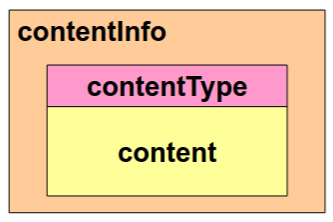
\includegraphics[width=0.4\textwidth]{img/cms structure.png}
  \label{fig:cms structure}
  \caption{CMS structure}
\end{figure}

\subsection{CMS content type}

There are different contentType available:

\begin{itemize}
    \item \textbf{data}: A generic sequence of bytes, serving as the
      base content.
    \item \textbf{signedData}: The data accompanied by one or more
      digital signatures (1..N), allowing parallel signing.
    \item \textbf{envelopedData}: The data encrypted using a symmetric
      algorithm, with the symmetric key encrypted for the intended
      recipient(s).
    \item \textbf{authenticatedData}: The data, a Message
      Authentication Code (MAC), and an encrypted key for
      recipient(s).
    \item \textbf{digestedData}: The data along with its cryptographic
      digest for integrity verification.
    \item \textbf{encryptedData}: The data encrypted using a symmetric
      algorithm, providing confidentiality.
\end{itemize}


\subsection{CMS contentType}
There are different contentType available:
\begin{itemize}
  \item Data: it is an encoding (with ASN.1) of a generic sequence of
    bytes. This is the basis.
  \item signedData: encoded data + parallel digital signatures, so a
    single document can have more signatures, which are called
    parallel, because all signatures compute the hash of the document,
    so the order of signing is not relevant, and they sign only the
    document. It is needed every time simultaneously signature of a
    document from more people is required.
  \item envelopedData: it contains the encrypted data (with a suitable
    symmetric algorithms) and then it also contains the key encrypted
    for recipient(s). It means that to decrypt the content you must be
    one of the valid recipients because the PKCS\#7 envelop also
    contains the key, which is encrypted with the public key so that
    only the valid recipients.
  \item authenticatedData: it contains the data with the MAC, and
    since MAC requires a shared key, but it is created by us, there is
    also the key encrypted for recipient(s). There is the assumption
    that the recipients have a public key, because that will be the
    way in which we will share with them the symmetric key used in the
    MAC.
  \item DigestedData: it is an unprotected format because it contains
    only the data plus the digest. It seems to be unprotected, but
    since this is a recursive format maybe then they will be used
    inside another format.
  \item encryptedData: contains the encrypted data with a symmetric
    algorithm, but it is assumed that the key has already been shared
    outside, so the key needed for decryption is not contained.
\end{itemize}


\subsection{CMS signed data}

\begin{figure}[H]
  \centering
  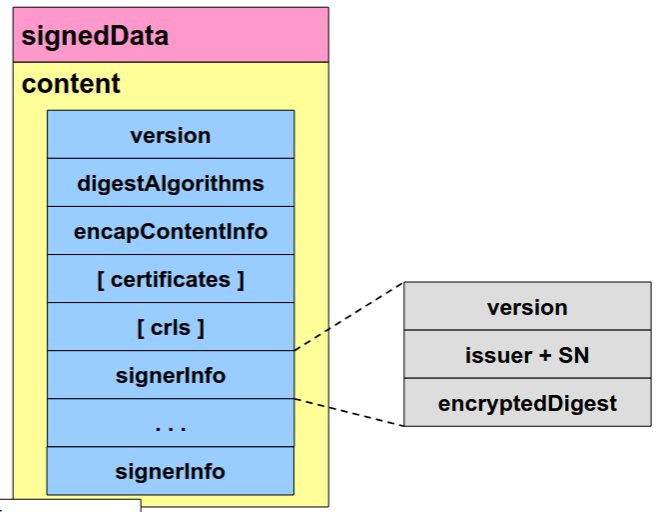
\includegraphics[width=0.4\textwidth]{img/cms signed data.png}
  \caption{CMS signed data}
\end{figure}
\subsection{CMS enveloped data}

\begin{figure}[H]
  \centering
  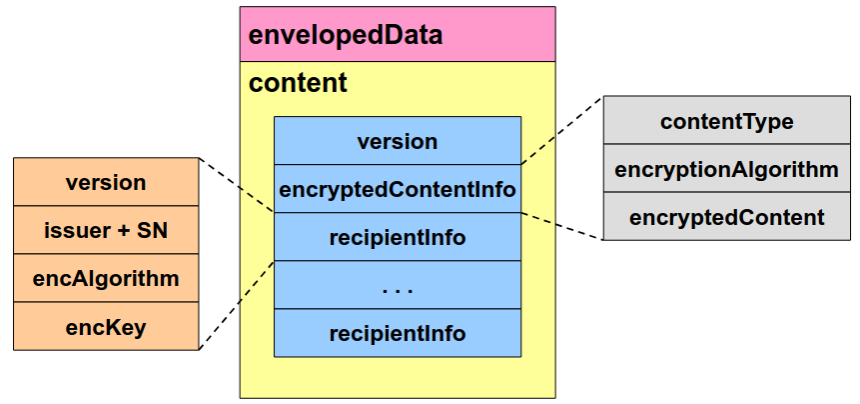
\includegraphics[width=0.4\textwidth]{img/cms enveloped data.png}
  \caption{CMS enveloped data}
\end{figure}
